\section{Demarche Expérimentale}

Le montage expérimental représenté à la figure \ref{fig:montage} permet de mesurer MA BITE REEEEEEEEEEEEEEEEEEEEEEEEEEEEEEEEEEEEEEEEEE

\begin{figure}
    \centering
    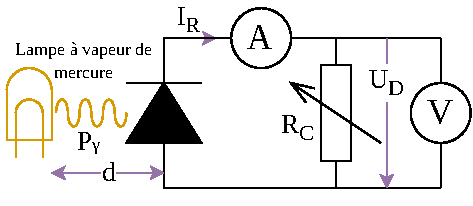
\includegraphics[width=12cm]{figures/montage.pdf}
    \caption{Diagramme électrique du montage expérimental \cite{notice} \cite{nicole}}
    \label{fig:montage}
\end{figure}

\begin{itemize}
\item Pas de liste du matériel!
\item Décrire de manière succincte la méthode et l'appareillage utilisés. 
\item Toutes les formules utilisées pour calculer les résultats doivent être énoncés clairement.
\item Préciser les conditions expérimentales: toutes les valeurs utilisées pour le calcul doivent être mentionnées at leur valeurs fournies.
\item Dans un article scientifique, toute la théorie et la description de la démarche expérimentale pour toutes les méthodes précèdent tous les résultats, puis une discussion donne la synthèse.
\item Citer les schémas si repris (aussi si vous utilisez les illustrations faites par vos collègues).
\end{itemize}